
\subsection{Estimator Fluctuations}
% As a neural net undergoing training can be modeled as a dynamical system relaxing towards a minimum energy state, there 
% may be some degree of `memory' in its state transition function resulting in hysteresis-like behavior of $\alpha$ as it 
% converges to its final value. Moreover, 
The estimator of $\alpha$ depends on a parameter $xmin$, which estimates $\lambda_{min}^{PL}$. In practice we often 
observe that two `competing' values of $xmin$ may have nearly equivalent $D_{KS}$, i.e., they may offer estimates of 
$\alpha$ that are of comparable quality with one another, but which result in wildly different $\alpha$ values. If we 
plot $\alpha$ over time, we often see it jumping between two independent curves. In layers close to the data, the 
data-driven HT behavior may win out, but in layers further from the data we often see this type of fluctuation. In such 
cases, the lower $\alpha$ is likely to be due to the influence of HT data rather than 

\begin{figure}[h]
    \centering
    
    \subfigure[$xmin$ over several epochs for several batch sizes]{
        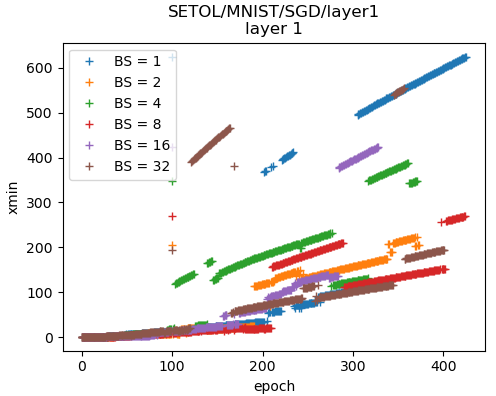
\includegraphics[width=4cm]{img/xmin-fluctuations.png}
        \label{fig:xmin_fluct}
    }
    \subfigure[$\alpha$ over several epochs for several batch sizes]{
        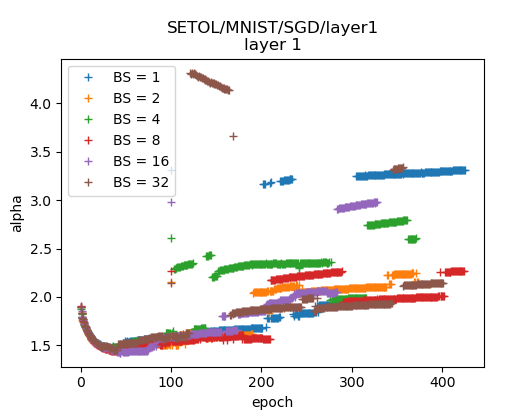
\includegraphics[width=4cm]{img/alpha-fluctuations.png}
        \label{fig:alpha_fluct}
    }
\\
    \subfigure[$\hat{\alpha}$ over several epochs for several batch sizes]{
        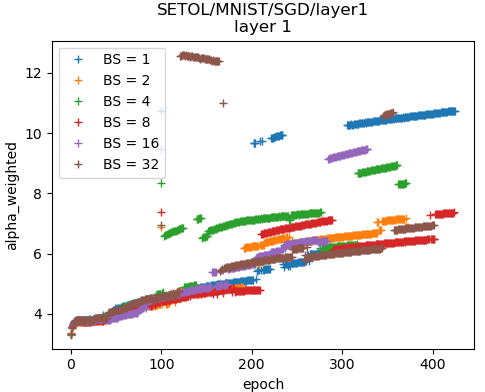
\includegraphics[width=4cm]{img/alpha-hat-fluctuations.png}
        \label{fig:alpha_hat_fluct}
    }
    \subfigure[$\lambda^{max}$ over several epochs for several batch sizes]{
        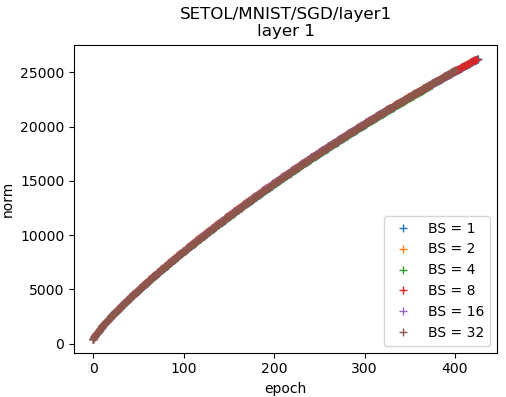
\includegraphics[width=4cm]{img/spectral-norm-fluctuations.png}
        \label{fig:norm_fluct}
    }

    \caption{Fluctuations in the value of $xmin$ (a), $\alpha$ (b), $\hat{\alpha}$ (c), and $\lambda^{max}$ (d) of a 
    weight matrix, over several epochs of training, for a variety of batch sizes. Note that for each, $xmin$ and 
    $\alpha$ remain relatively stable before and after each jump, as a different $xmin$ value dominates the calculation.
}
 \label{fig:fluctuations}
\end{figure}


In Figure \ref{fig:fluctuations}, values of $xmin$, $\alpha$, $\hat{\alpha}$ and $\lambda^{max}$ are shown for each 
epoch over a training run, for a variety of batch sizes. (See Section \ref{sxn:empirical} and appendix \nred{XXX}.) As 
$xmin$ jumps from one value to another, so does $\alpha$. Each such jump indicates the sudden transition of one part of 
the tail becoming dominant over another, resulting in a different value of $\alpha$. When interpreting $\alpha$, 
fluctuations in $xmin$ should be taken into account.
\nred{If we include this plot, it belongs in the experimental section on the hystersis curves; To replace this, I recokmend using the plots I suggested in the Dicsord channel, which shows cases where the PL fits are tricky, using the weightwatcher tool}



\begin{figure}[b] %[h]                                                                                                                                                         
    \centering
    \subfigure[Log-Log ESD]{
      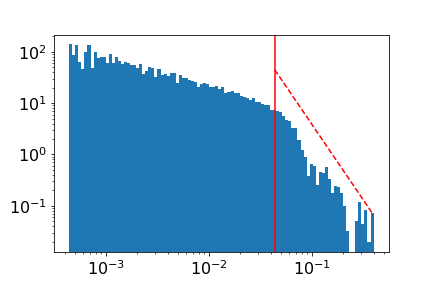
\includegraphics[width=3cm]{./img/fig1-2a.png}
    }
    \subfigure[Lin-Lin ESD]{
      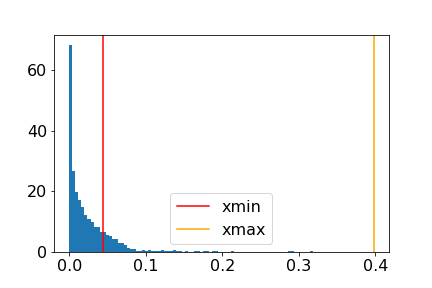
\includegraphics[width=3cm]{./img/fig1-2b.png}
    }
    \subfigure[Log-Lin ESD]{
      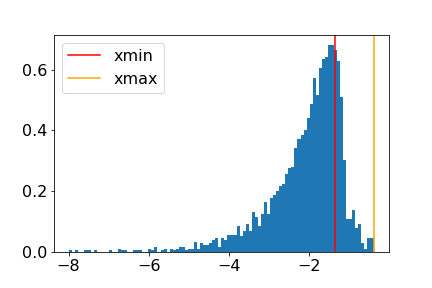
\includegraphics[width=3cm]{./img/fig1-2c.png}
    }
    \subfigure[$\lambda_{min}$ vs KS distance]{
      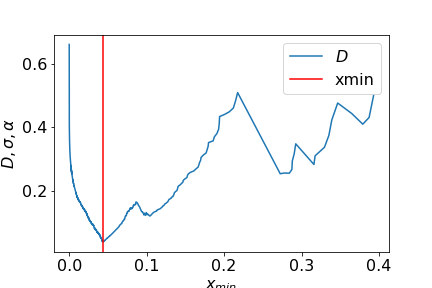
\includegraphics[width=3cm]{./img/fig1-2d.png}
    }
    \subfigure[Log-Log ESD]{
      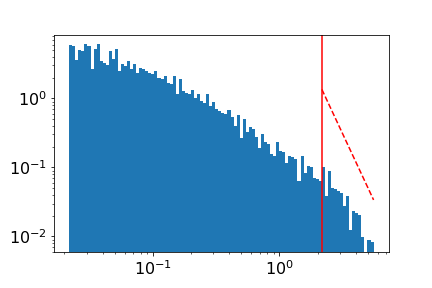
\includegraphics[width=3cm]{./img/fig1-3a.png}
    }
    \subfigure[Lin-Lin ESD]{
      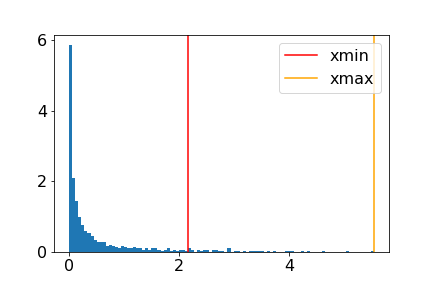
\includegraphics[width=3cm]{./img/fig1-3b.png}
    }
    \subfigure[Log-Lin ESD]{
      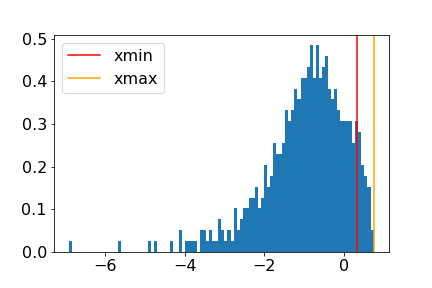
\includegraphics[width=3cm]{./img/fig1-3c.png}
    }
    \subfigure[$\lambda_{min}$ vs KS distance]{
      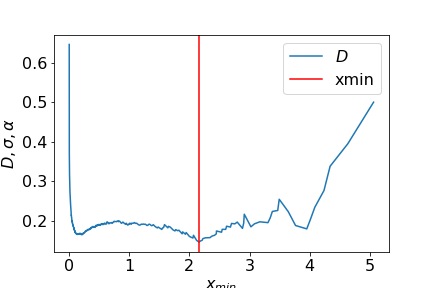
\includegraphics[width=3cm]{./img/fig1-3d.png}
    }
    \caption{Difficult PL fits}
  \label{fig:hard-pl-fits}
\end{figure}

